%%%%%%%%% PROPOSAL -- 15 pages (including Prior NSF Support)
% From the NSF Grants Proposal Guide:
% "The Project Description should provide a clear statement of the work 
% to be undertaken and must include: objectives for the period of the proposed 
% work and expected significance; relation to longer-term goals of the PI's 
% project; and relation to the present state of knowledge in the field, 
% to work in progress by the PI under other support and to work in progress 
% elsewhere."

%\required{Project Description}
\section{Project Description}

\subsection{Agenda}

\subsubsection{Algorithms / Programming}
In doing some of our own research, it seems like Simulated Annealing is a common
approach or suggetstion for optimizing biomechaical models \cite{mcgowan} 
\cite{thelen} \cite{lloyd}, so the project will 
choose \textbf{generational} methods of GAs. Generational methods tend to get 
rid of variability in potential models, similar to how Simulated Annealing 
simply never sees them. If the Generational method doesn't work well, a 
\textbf{steady state} approach will be tried. Each can be tried with 
combinations of mutation rates, crossover rates, and selection values.

The generational approach has another simularity to Simulated Annealing, in 
that it tends to find local optimums faster. Hopefully the project will be
able to use the benefits of this, without getting stuck at local optimums. 
The generational approach can be enhanced by using Age Layered Populations
(ALPs), or an age limit for every model. This would be an interesting 
feature to experiment with, and would be a minor addition to our current
GA code base.

Both approaches will use a \textbf{population size} starting with $ P = 500 $. 
\textbf{Crossover} methods will be picked from two point and uniform. 
For crossover, the best individuals will be selected using a rank based / 
tournament \textbf{selection function}. A random sample of $ k $ individuals
will be selected, starting with 10. $ k $ will be increased if solutions are
not converging quickly enough (restricts population variability), and k will be
decreased if population solutions seem to get stuck in local optimums. This
was the best approach in previous projects, for similar seach spaces.

\begin{figure}[!h]
        \begin{center}
		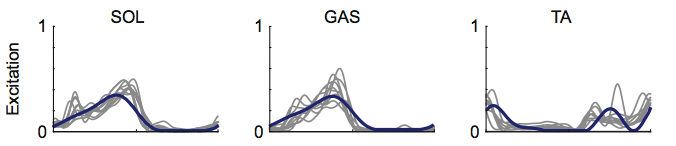
\includegraphics[width=120mm]{images/excite}
               \caption{Sample muscle excitations and optimizations \cite{mcgowan}}
                \label{curves}
        \end{center}
\end{figure}

The output curves (see samples in Figure \ref{curves}) seems to be 
realitively smooth, but perhaps less predictable than the typical GA benchmarks.
This means we may be have to keep the value of $ k $ low to avoid local 
optimums. But it is our first priority to come up with really good 
solutions in reasonable time. The current results look inaccurate 
compared to the results in previous projects using GA's, so we're anticipating
some hidden complexities and lots of local optimums to overcome in optimization.
These have probably foiled Simulated Annealing a bit.

\begin{comment}
\subsubsection{Parallel Programming}

Parallel Programming means doing many similar things in software at once.
In parallelizing these algorithms, the project will identify some of the
concepts in parallel programming. These concepts will be challenging. But,
the project will explain these concepts to scientists and mathematicians first;
not computer scientists. The goal of the project is to provide reference and
guidelines for non-computer scientists. 

These concepts include:
\begin{itemize}
	\item Data parallelism
	\item Task parallelism
	\item Pipeline parallelism
	\item Mutual Exclusion issues
	\item Data dependency
	\item Process granularity
	\item Process profiling
\end{itemize}

The goal of the project is not to explain the computer science concepts in
depth. Instead, they will cover the breadth of these concepts, and explain them
in the least technical way possible. The project will provide as much practical
information to non-savvy readers as possible. These readers will hopefully be 
scientists and mathematicians about to start their own projects. The entire
process of writing HPC software will be the focus.
\end{comment}


\subsection{Methodology}
The development for the project will start with replacing the current 
Simulated Annealing function in Dr. McGowan's code base with our own GA 
interface. Simulated Annealing will probably be run side by side with the GA
until it is determined that the GA performs better. If the GA outperforms 
Simulated Annealing, then Simulated Annealing will be left out. Generational 
and steady state approaches will both be tried. Once a better method is found,
performance improvements will sought, including candidate tasks for 
paralllelism.

If parallelism proves to be theoritically beneficial, it will be documented, 
and may be implemented. Simulations will be run at first on a few multicore 
machines, and if speed-ups warrant, may be run on small to medium size 
compute clusters. It is our experience that model evaluation / fitness 
functions are where parallelism becomes possible and beneficial. But our 
experience is that large speed-ups are not common.

If the GA and performance evaluation portions of the project are successful,
then the project will attempt to enhance the fitness / evaluation function 
(called the 'objective' function in Dr. McGowan's research). Dr. McGowan will
often change parameters very slightly for the evaluation function, in an 
attempt to represent the rea world biomechanical model with this evaluation 
fuction. A GP would probably be a good approach. Time may not permit this much
work, but would be a good future task for future research.

\subsubsection{Existing Software}
Dr. McGowan has made available to our project a code base that is currently
running his optimizations. This code is written in C++ using Microsoft's 
Visual Studio, and interfaces with the 3d simulation software and MatLab to
show optimization results. MatLab may be a challenge to our project, so some
open source language like R might be our option to compare optimization 
results. The Simulated Annealing optimization will be replaced with our EC
interface, and this will hopefully be the only other alteration.

\subsubsection{Project Software}
Our software will probably be written in C++. Our current GA code base is 
written in R, and will have to be adapted to C++. Our current GP code base is
in C++, so it won't require much adaptation. The proposed project code will 
work in Dr. McGowan's current development environment without any changes.

\section{Workplan}

\subsection{Schedule}

\begin{tabular}{ l r }
  November 11th - 15th		& Project proposal \\
  November 16th - 18th 		& Current code base experimentation \\
  November 19th - 23rd 		& GA implementation\\
  November 24th - 25th 		& Performance analysis\\
  November 26th - 30th 		& Performance enhancement and GP analysis\\
	
\end{tabular}


\section{Statement of Qualifications}
This project is an application of 1 semester of Evolutionary Computation study.
Further experience of evolving systems is taken from another semester of 
Artificial Intelligence. The biological software development and performance
analysis experience comes from 2+ years working in the University of Idaho 
IBEST Computing Core, as well as from experience from NCMGRP, a research 
project lead by Ph. D. student Adam Wells at the University of Idaho College of 
Natural Resources. This research project focuses on spatial analysis of animal
movement throughout the northwest.

\section{Conclusion}
In conclusion, Dr. McGowan's research is important because it helps us
understand the mechanics of motion in the body. Results from his research
good apply to anything from CGI in video games to adaptive prostetics for
humans. Getting usable results from the research could come down to having 
a good optimization. It is therefore important to develop better optimization
over Simulated Annealing, as Simulated Annealing has left a lot of room for
improvement. It may or may not make sense to GA's or GP's over other methods
(like Artificial Neural Networks), considering what the actual biomechanical
system does. But an evolutionary optimizations like GAs or GPs almost 
certainly should offer improvements over more static optimizations, like
Simulated Annealing. 

%\required{Broader Impacts}
% as in the project summary, broader impacts must be called out separately 
% in the project description.  You may be able to give more specific
% examples, or discuss how you've previously achieved these impacts.
% It should be similar, but not identical, to the Broader Impacts statement
% in the project summary

%\required{Results From Prior NSF Support}
% 5 pages or fewer of the 15 pages for entire description document.
% include results from NSF grants received in the past 5 years.
% if supported by more than one grant, choose the most relevant one
% for each grant, include: NSF award number, amount, dates of
% support, and publications resulting from this research.
% due to space limitations, it is often advisable to use citations rather
% than putting the titles of the publications in the body 
% of this section

% e.g.: "My prior grant, "Uses of Coffee in Mathematical Research" (DMS-0123456, 
% $100,000, 2005-2008), resulted in 3 papers [1],[2],[3], demonstrating..."

% if requesting postdoctoral research salary, a supplemental 1-page document
% called "Postdoc Mentoring Plan" will be required 

